\documentclass{article}
\hyphenation{op-tical net-works semi-conduc-tor}
\usepackage{amsthm, tikz}
\usepackage[ruled,noline, linesnumbered,noend]{algorithm2e}
\usetikzlibrary{automata,calc}
\usetikzlibrary{arrows}
\usepackage{amssymb}
\usepackage{mathtools}
\usepackage{hyperref}

\begin{document}
\title{Controller Synthesis for Timed Systems}

\def\cpre{\textrm{\sf CPRE}}
\def\post{\textrm{\sf Post}}
\def\predc{\textrm{\sf Pred}_c}
\def\predt{\textrm{\sf Pred}_{\geq 0}}
\def\predu{\textrm{\sf Pred}_u}
\def\calQ{\mathcal{Q}}
\newcommand*\out{\textsf{Outcome}}
\newcommand*\state{\textsf{state}}
\newcommand*\trans{\textsf{trans}}
\newcommand*\TA{\ensuremath{\mathcal{A}}}
\newcommand\runs{\textrm{\sf Runs}}
\newcommand*\Act{\ensuremath{\mathsf{Act}}}
\newcommand*\Locs{\mathcal{L}}
\newcommand*\Realnn{\mathbb{R}_{\geq 0}}
\newcommand*\Clocks{\mathcal{C}}
\newcommand*\Clocksz{\mathcal{C}_0}
\newtheorem{theorem}{Theorem}[section]
\newtheorem{definition}[theorem]{Definition}
\newtheorem{conjecture}[theorem]{Conjecture}
\newtheorem{problem}[theorem]{Problem}
%\newtheorem{proposition}[theorem]{Proposition}
%\newtheorem{property}[theorem]{Property}
%\newtheorem{corollary}[theorem]{Corollary}
\newtheorem{lemma}[theorem]{Lemma}
\newtheorem{remark}[theorem]{Remark}
\newtheorem{example}[theorem]{Example}
%\newtheorem{notation}[theorem]{Notation}
\newtheorem{notation}{Notation}{\bfseries}{\itshape}
% make the title area
\maketitle

\begin{abstract}
  Controller synthesis considers \emph{open} systems where 
  some actions are \emph{controllable}, while others are \emph{uncontrollable},
  and the goal is to automatically synthesize a policy to enable or disable
  controllable actions so as to ensure that the overall behaviors of the system
  satisfy a given specification. In this tutorial, we describe some data structures 
  and algorithms that are used for the controller synthesis of timed systems.
\end{abstract}


\section{Introduction}
While \emph{formal verification} consists in verifying that \emph{all} behaviors of a
given system model satisfies a given specification, \emph{controller synthesis}
consists in constructing systems that satisfy their specifications by
construction.
In controller synthesis, one is interested in \emph{open systems} which are 
non-deterministic systems that are
not entirely specified; they contain \emph{uncontrollable actions} which model
the actions coming from the environment (upon which one has no control), and
\emph{controllable actions} which can be enabled or disabled by a controller.
The main problem consists in synthesizing (\textit{i.e.} automatically
computing) a control policy which enables/disables controllable actions at all
states so as to guarantee a given specification.

We concentrate on \emph{timed systems} which are essentially discrete systems
where time delays in the executions are explicitly modeled. We will consider
the \emph{timed automata} formalism~\cite{AD-tcs94}, in which time can be
modeled as either continuous, where time delays are arbitrary real numbers, or
discrete, where time delays are integers. We consider the continuous-time view
in this paper, but both views are complementary and have 
their advantages. We give a quick comparison in the last section.

\textbf{Some References}
Controller synthesis problems have been studied extensively in the so-called
discrete-event systems community~\cite{rw-1989}; see also~\cite{CL-book06} for
an introduction. The theory has been studied both in the discrete-time and
continuous-time settings. Controller synthesis was also studied from a
game-theoretic perspective in terms of two-player games played on
graphs where the player controller plays against an adversarial environment
player~\cite{PR-popl89,ALW89,Dill89}.
Winning strategies for the controller then correspond to control
policies ensuring the specification. 
Controller synthesis problems for continuous-time models formalized as games
played on timed automata were 
studied in~\cite{AMP-concur98,AMPS98}; several efficient algorithms were
given, and tools were developed~\cite{TA-fm99,altisen2002tools,Cassez05}.
The problem has also been studied for time Petri nets~\cite{gardey2006safety}.

\section{Example}
Before giving any formal definition, we illustrate the timed automata formalism and the controller synthesis
problem on a simple railroad switch controller model.

Informally, timed automata are finite automata enriched with a finite set of analog clock
variables which are used to measure time. 
All clocks are assumed to be synchronous, and they can only grow with a constant rate; they can only be reset
during transitions. A timed automaton is given in Figure~\cref\{fig:ter}, where
the underlying finite automaton describes the different modes of the train. 
The train is initially at location \texttt{idle}, meaning it is far from the
railroad switch. The clock~$x$
is reset upon entering the state \texttt{close}, and the next transition
(to \texttt{arrived}) can only happen between 20 and 30 time units, which
depends on the actual speed of the train, and cannot be controlled by the
switch. 
We denote uncontrollable events by dashed arrows and full arrows show
controllable transitions.
Once in the arrived state, the train can enter the \texttt{crossing} state
between 1 and 2 time units, unless a controllable action was sent by the switch
in at most 1 time unit, in which case the train enters the \texttt{stopping}
state. From the latter state, only the switch can order the train into the
\texttt{crossing} state.

Notice that the behavior of the train is uncontrollable within given time
constraints except for the stop and go actions. This means that from the railroad
switch controller's perspective, we have no control on the exact behavior of the
train; but we only know lower and upper bounds on its speed. The railroad switch
controller can only order the train to stop, in the \texttt{arrived} state, and release it by a go
command.

\begin{figure}[ht]
	\centering
  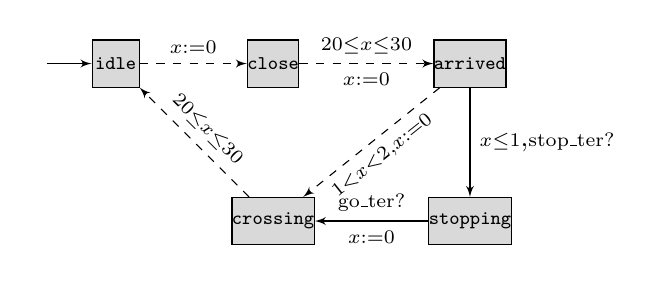
\begin{tikzpicture}[node distance=2cm,auto]
		\tikzstyle{every state}=[rectangle,fill=black!15,minimum size=17pt,inner sep=0pt]
		\node (preA) at (0,0) {};
    \node[state] at (1,0) (A) {\texttt{\scriptsize idle}};
    \node[state,right of=A] (B) {\texttt{\scriptsize close}};
    \node[state,node distance=2.5cm, right of=B] (C) {\texttt{\scriptsize arrived}};
    \node[state,below of=B] (Cr) {\texttt{\scriptsize crossing}};
    \node[state,below of=C] (St) {\texttt{\scriptsize stopping}};
    \everymath{\scriptstyle}
    \path[-latex'] 
      (preA) edge (A)
      (A) edge[dashed] node[above] {$x:=0$} (B)
      (B) edge[dashed] node[above] {$20\leq x\leq 30$} node[below]{$x:=0$}(C)
      (C) edge node[right]{$x\leq 1$,\scriptsize  stop\_ter?} (St)
      (C) edge[dashed] node[below,sloped]{$1<x< 2,x:=0$} (Cr)
      (St) edge node[above] {\scriptsize go\_ter?} node[below]{$x:=0$} (Cr)
      (Cr) edge[dashed] node[above,sloped]{$20\leq x\leq 30$} (A);
  \end{tikzpicture}
  \caption{The TER model.}
  \label{fig:ter}
\end{figure}

Assume now that another train is to use the same railroad switch, and assume
that it is now a TGV. Figure~\cref\{fig:tgv} describes this model which is almost
the same as the TER one, except that TGVs travel much faster.

\begin{figure}[ht]
	\centering
  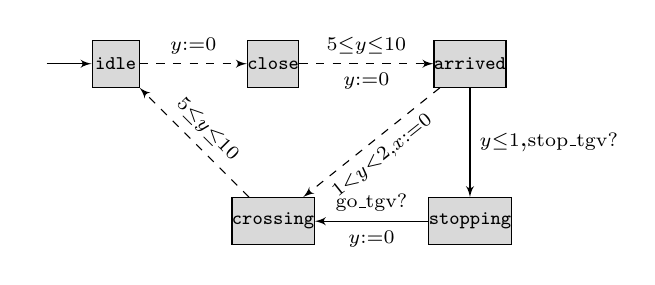
\begin{tikzpicture}[node distance=2cm,auto]
		\tikzstyle{every state}=[rectangle,fill=black!15,minimum size=17pt,inner sep=0pt]
		\node (preA) at (0,0) {};
    \node[state] at (1,0) (A) {\texttt{\scriptsize idle}};
    \node[state,right of=A] (B) {\texttt{\scriptsize close}};
    \node[state,node distance=2.5cm, right of=B] (C) {\texttt{\scriptsize arrived}};
    \node[state,below of=B] (Cr) {\texttt{\scriptsize crossing}};
    \node[state,below of=C] (St) {\texttt{\scriptsize stopping}};
    \everymath{\scriptstyle}
    \path[-latex'] 
      (preA) edge (A)
      (A) edge[dashed] node[above] {$y:=0$} (B)
      (B) edge[dashed] node[above] {$5\leq y\leq 10$} node[below]{$y:=0$}(C)
      (C) edge node[right]{$y\leq 1$,\scriptsize  stop\_tgv?} (St)
      (C) edge[dashed] node[below,sloped]{$1<y< 2,x:=0$} (Cr)
      (St) edge node[above] {\scriptsize go\_tgv?} node[below]{$y:=0$} (Cr)
      (Cr) edge[dashed] node[above,sloped]{$5\leq y\leq 10$} (A);
  \end{tikzpicture}
  \caption{The TGV model.}
  \label{fig:tgv}
\end{figure}

Our system is now composed of these two timed automata, which means that they are
executed in parallel: the clocks $x$ and~$y$ grow synchronously, and each
automaton can make a transition independently from the other one.

We would like to synthesize a controller for the railroad switch so as
to avoid any accident: we would like to make sure that the two trains are never
in the crossing state at the same time.
Intuitively, the controller should stop one of the trains whenever there is risk
of collision. We would like to synthesize this controller as a timed automaton,
that will observe the states of the two trains, and send the signals
$\{$stop\_ter, go\_ter, stop\_tgv, go\_tgv$\}$ accordingly. Then \emph{all}
behaviors of the system controlled by this controller will satisfy the
specification, which is that both trains are never crossing at the same time.

This tutorial shows how to compute such strategies algorithmically. At the end
of the paper, we describe a strategy synthesized for this problem using a
software tool.
\section{Controller Synthesis in Finite-State Spaces}
Let us first explain the principle of controller synthesis for finite-state
systems which are simply finite automata (with no clocks). We will then extend
these ideas in later sections to continuous state spaces using timed automata.

\paragraph{Problem Description}
We define a \emph{finite game} as a tuple $G = (\Locs, \ell_0, E_u, E_c)$, where~$\Locs$ is
the set of locations, $\ell_0$ is the initial location, $E_u$ and~$E_c$ are
respectively uncontrollable and controllable edges with $E_u,E_c \subseteq
\Locs \times \Locs$. A \emph{run} of a finite game is a sequence $q_1q_2\ldots$
where~$q_1 = \ell_0$, and~$(q_i,q_{i+1}) \in E_u \cup E_c$.
We assume that from each location~$\ell$ there is a controllable transition, 
that is $\exists \ell', (\ell,\ell') \in E_c$.
A \emph{control strategy} is a function $\Locs \rightarrow
E_c$.\footnote{Knowledgeable readers will notice that we only consider
\emph{positional} (a.k.a. memoryless) controllers here.}.

Intuitively, when the system, described by the finite game, is controlled by the
control strategy~$f$, at each location~$\ell$, the only possible
transitions are $f(l)$ or any uncontrollable transition from~$E_u$.
Let~$\out_f(\TA)$ denote the set of such runs.

We concentrate on \emph{safety specifications}: assume that the controller wants to avoid a
subset~$B \subseteq \Locs$ of the state space. We say that strategy~$f$
is a \emph{winning strategy for $B$} if no run of~$\out_f(\TA)$ visits a
location from~$B$.
The \emph{finite-state safety control} decision problem is defined as follows.
\begin{problem}[Finite-state Safety Control]
  Given a finite game~$\TA=(\Locs,\ell_0,E_u,E_c)$ and states~$B \subseteq
  \Locs$, is there a control strategy~$f$ that is winning for~$B$?
\end{problem}

If the answer is positive, we are also interested in actually
computing a control strategy.


\paragraph{Solution}
We will show how to decide whether the controller has a winning strategy to
avoid~$B$. We will construct such a strategy by first ensuring that $B$ is
avoided in one step, then in two steps, and so on.

Let us define the set of states from which the
controller can ensure to reach some state of a set~$C$ in one step. This is called the set of
\emph{controllable predecessors} of~$C$, and defined as follows:
\[
  \begin{array}{ll}
  \cpre(C) = C \cap \{ \ell &\mid \forall \ell', (\ell,\ell') \in E_u \Rightarrow \ell'
  \in C,\\& \land \exists \ell', (\ell,\ell') \in E_c, \ell' \in C\}.
\end{array}
\]

Now, $\cpre(\Locs \setminus B)$ is the set of states from which the controller
has a strategy to avoid~$B$ for one step, and more generally, it can avoid~$B$
for $k$ steps starting from any state of $\cpre^k(\Locs\setminus B)$.
Notice that $k \mapsto \cpre^k(\Locs\setminus B)$ is non-increasing for the set
inclusion and is bounded below. Moreover, the state space is finite, which means
that the limit $\lim_{k\rightarrow \infty} \cpre^k(\Locs\setminus B)$ exists and
is reached in a finite number of times. Formally,

\begin{theorem}
  For any finite game~$G = (\Locs, \ell_0, E_u, E_c)$ and a safety
  specification~$B\subseteq \Locs$, $\cpre^*(\Locs\setminus B) =
  \lim_{k\rightarrow \infty}\cpre^k(\Locs\setminus B)$ exists and is the set of
  locations from which the controller has a winning strategy for~$B$.
\end{theorem}

Once the set $W = \cpre^*(\Locs\setminus B)$ is computed, a winning strategy can be
extracted easily: for each location~$\ell \in W$, we define $f(\ell) = \ell'$ such
that $(\ell,\ell') \in E_c$ and $\ell' \in W$; such a location exists by the
definition of~$\cpre$ and the fact that~$W$ is a fixpoint: $W = \cpre(W)$.

\section{Controller Synthesis for Timed Automata}
To formalize controller synthesis problems for timed
systems, we define \emph{timed games} which are games played on timed
automata~\cite{AD-tcs94}. We mostly follow the definitions of~\cite{Cassez05}.

\paragraph{Timed Automata and Games}
% We fix a finite set~$\Clocks$ of clock variables, we~call \emph{valuations} the
% elements of~$\Realnn^\Clocks$. For a subset $R\subseteq \Clocks$ and a
% valuation~$\nu$, ${\nu[R \leftarrow 0]}$~is the valuation defined by
% ${\nu[R \leftarrow 0](x) = 0}$ if $x \in R$ and ${\nu[R\leftarrow
%     0](x) = \nu(x)}$ otherwise. Given $d \in \mathbb{R}_{\geq 0}$ and
% a valuation $\nu$, the valuation $\nu+d$ is defined by $(\nu+d)(x) =
% \nu(x)+d$ for all $x\in \Clocks$. We~extend these operations to sets
% of valuations in the obvious way. We write $\vec{0}$ for the valuation
% that assigns~$0$ to every clock.

% An atomic clock constraint is a formula of the form $k \preceq x \preceq' l$
% or $k \preceq x - y \preceq' l$ where $x,y \in \Clocks$, $k,l \in
% \mathbb{Z}\cup\{-\infty,\infty\}$ and ${\mathord\preceq,\mathord\preceq' \in
% \{\mathord<,\mathord\leq\}}$.  A~\emph{guard} is a conjunction of
% atomic clock constraints.
% A~valuation~$\nu$ satisfies a guard~$g$, denoted $\nu \models g$,
% if all constraints are satisfied when each $x\in \Clocks$ is replaced
% with~$\nu(x)$.
% We~write $\Phi_\Clocks$ for the set of guards built on~$\Clocks$.
% A~\emph{zone} is a subset of~$\Realnn^\Clocks$
% defined by a guard.

% A~\emph{timed game} $\TA$
% is a tuple $(\Locs,\Act, \Clocks,\penalty0 \ell_0,E_u,E_c)$, where $\Locs$
% is a finite set of locations, $\Clocks$~is a finite set of clocks, $E_c,E_u
% \subseteq \mathcal{L} \times \Phi_\Clocks \times \Act \times 2^\Clocks
% \times \mathcal{L}$ are sets of controllable and uncontrollable edges
% respectively, and $\ell_0\in \Locs$ is the
% initial location.
% An~edge $e = (\ell,g,a,R,\ell')$ is also written as
% $\ell \xrightarrow{g, a , R} \ell'$, and represents a transition from
% location~$\ell$ to~$\ell'$, with guard~$g$, action label~$a$, and clock reset
% set~$R$.
% A \emph{state} is a
% pair $q=(\ell,\nu)\in \Locs\times \Realnn^\Clocks$.
% We write $\calQ = \Locs \times \Realnn^\Clocks$.
% An edge $e = (\ell,g,a,R,\ell')$ is enabled in a state $(\ell,\nu)$ if
% $\nu$ satisfies the guard $g$.
% There is a \emph{transition from state~$(\ell,\nu)$ to state~$(\ell',\nu')$ through
% edge~$e = (\ell,g,a,R,\ell')$} if $\nu \models g$, $\nu' = \nu[R\leftarrow 0]$.
% In this case, we write $(\ell,\nu) \xrightarrow{e} (\ell',\nu')$.
% Let~$E_c(\ell)$ denote the set of edges in~$E_c$ that leave the location~$\ell$,
% and define~$E_u(\ell)$ similarly.

The set of possible behaviors of a timed automaton can be described by the set
of its runs, as follows.
A~\emph{run} of~$\TA$ is a sequence $\rho = q_1e_1q_2e_2\ldots$ where $q_i \in
\calQ$
and writing $q_i = (\ell,\nu)$, either $e_i \in \mathbb{R}_{>0}$, in which case $q_{i+1}
= (\ell,\nu + e_i)$, or
$e_i =(\ell,g,a,R,\ell')\in E$, in which case 
$q_i \xrightarrow{e_i} q_{i+1}$.
For a run~$\rho$ defined as above, we write~$\state_i(\rho) = q_i$, 
and $\trans_i(\rho) = e_i$.
A run is \emph{maximal} if it is an infinite sequence or if it cannot be
extended by a controllable action, that is, no controllable edge is enabled
after any delay from the last state.

A~\emph{strategy} for a timed automaton is a 
function~$f : \calQ \rightarrow E_c\cup\{\epsilon\}$.
Intuitively, at any state~$q=(\ell,\nu)$, the controller that applies
strategy~$f$ waits if $f(q)=\epsilon$, and takes the edge~$f(q) \in E_c$
otherwise.

The set of \emph{outcomes} of the timed automaton~$\TA$ \emph{under
strategy~$f$} is defined as the set of maximal runs~$\rho$ such that
\begin{enumerate}
  \item $\state_1(\rho) = (\ell_0,\vec{0})$,
  \item for all~$i\geq 1$ such that~$\trans_i(\rho) \in E$, we have either
  $\trans_i(\rho) \in E_u$, or $\trans_i(\rho)
  = f(\state_i(\rho)) \in E_c$.
  \item for all~$i\geq 1$ such that~$\trans_i(\rho) \in \Realnn$, for all~$t \in
  [0,\trans_i(\rho))$, $f(\state_i(\rho) + t) = \epsilon$.
\end{enumerate}
In words, (1)~an outcome under~$f$ starts in the initial state; (2)~at any moment,
any enabled uncontrollable transition or any controllable transition prescribed
by~$f$ can be taken; and (3)~if the outcome contains a positive delay, then the strategy~$f$ 
prescribes waiting at any state traversed during the delay -except possibly for the
last state.

\paragraph{Timed Controller Synthesis}
We consider a timed game~$\TA = (\Locs,\Act,\Clocks,\penalty0 \ell_0,E_u,E_c)$
and a safety specification~$B \subseteq \calQ$. As for the finite-state case,
a strategy in~$\TA$ is winning for~$B$ if no outcome of~$\TA$ compatible
with~$f$ visits~$B$. We define the problem formally as follows.

\begin{problem}[Timed Safety Control]
   Given a timed game~$\TA = (\Locs,\Act,\Clocks,\penalty0 \ell_0,E_u,E_c)$ 
   and a set~$B \subseteq \calQ$, is there a control
   strategy~$f$ that is winning for~$B$?
\end{problem}

We are going to follow the algorithm for the finite-state case and define
controllable predecessors, but this needs some care due to delay transitions in
timed automata.

We define the set of \emph{safe time-predecessors} to reach~$X \subseteq \calQ$ while
avoiding~$Y \subseteq \calQ$ as follows:
\[
  \begin{array}{ll}
    \predt(X,Y) = \{q \in \calQ &\mid \exists d\geq 0, q+d \in X,\\
      &~ \land \forall d' \in[0,d), q+d' \not \in Y\}.
  \end{array}
\]
In words, from any state of $\predt(X,Y)$, the state~$X$ can be reached by
delaying while never crossing~$Y$ on the way. 
For any $X \subseteq \calQ$, let us denote
\[\predc(X) = \{ (\ell,\nu) \in \calQ \mid \exists e \in E_c(\ell), 
\exists q' \in X, (\ell,\nu) \xrightarrow{e} q'\},\]
that is the set of immediate predecessors of~$X$ by edges in~$E_c$.
We define symmetrically $\predu(X)$ using~$E_u$ instead of~$E_c$.
The controllable predecessors
operator for timed systems is defined as follows:
\[
  \pi(X) = \predt(\predc(X), \predu(\calQ \setminus X)).
\]
Intuitively, from any state of~$X$, the controller can wait until it can fire a controllable
transition back into~$X$, while any uncontrollable transition that might happen
while waiting remains inside~$X$.
Hence, this operator allows us to express the states that can be controlled
within one step. The following theorem shows that the greatest fixpoint of this
operator exists and can be computed. It follows from~\cite{AMPS98,AMP-concur98}.

\begin{theorem}
   \label{thm:timed-control}
   For any timed game~$\TA$ and safety specification~$B \subseteq \calQ$, 
   $\pi^*(\calQ\setminus B) = \lim_{k \rightarrow \infty} \pi(\calQ\setminus B)$ exists, is reached 
   in a finite number of steps. This limit is precisely the set of states from
   which the controller has a winning strategy for the specification~$B$.
\end{theorem}

\section{Data Structure: Difference-Bound Matrices}
While Theorem~\cref\{thm:timed-control} gives a characterization of winning states for the
controller, it does not immediately allow one to actually decide whether a given
state is winning. In fact, we need to provide a data structure to represent the
subsets of~$\calQ$, on which controllable predecessors can be applied.

We introduce \emph{difference-bound matrices} which define convex polyhedra inside $\Realnn^\Clocks$
and are one of the data structures that are used in timed automata
verification~\cite{Dil90,BM83}. The idea is to write down an upper bound
on each clock, and on the difference of each clock. Formally, given a clock
set~$\Clocks=\{x_1,\ldots,x_m\}$, define $\Clocksz = \Clocks \cup \{x_0\}$
where~$x_0$ is seen as a
special clock which is always~$0$ (this is just to simplify the subsequent notations). Now,
a difference-bound matrix (DBM) is a $|\Clocksz|\times |\Clocksz|$ matrix
with coefficients in $\{\leq,<\} \times \mathbb{N}$. For any DBM~$M$, 
the $i,j$-component of the matrix~$M$ will be written
$(\prec^M_{i,j}, M_{i,j})$ where $\prec^M_{i,j}$ is the inequality, and
$M_{i,j}$ the integer coefficient. The DBM~$M$ defines the zone~$[M]$ defined by
the following constraints:
\[
  [M] := \bigwedge_{0\leq i,j \leq |\Clocksz|} x_i-x_j \prec^M_{i,j} M_{i,j}.
\]

\begin{example}
  Consider the clock set $\Clocks=\{x_1,x_2\}$, and recall we define~$x_0=0$.
  Consider the zone $Z$ defined by the conjunction of clock constraints 
  $x_1\leq 1 \land x_1-x_2 \leq 0 \land x_2\leq 3\land x_2-x_1 \leq 2$, which can be
  written as the following DBM:
  \[
    \begin{pmatrix}
      (0,\leq)&(0,\leq)&(0,\leq)\\
      (1,\leq) &(0,\leq)&(0,\leq)\\
      (3,\leq)&(2,\leq)&(0,\leq)
    \end{pmatrix}
    \qquad
  \tikz{
    \path[use as bounding box] (-1,0.5) -- (2,1.5);
    \begin{scope}[scale=.4]
      \fill[gray] (0,0) -- (1,1) -- (1,3) -- (0,2) -- cycle;
      \draw[-latex',line width=.6pt] (0,0) -- (3.5,0) node[right] {$x_1$};
      \draw[-latex',line width=.6pt] (0,0) -- (0,3.5) node[left] {$x_2$};
      \begin{scope}[line width=0.1pt]
      \draw[-] (1,0) -- (1,3.5);
      \draw[-] (2,0) -- (2,3.5);
      \draw[-] (0,1) -- (3.5,1);
      \draw[-] (0,2) -- (3.5,2);
      \draw[-] (0,0) -- (3.5,3.5);
      \draw[-] (1,0) -- (3.5,2.5);
      \draw[-] (2,0) -- (3.5,1.5);
      \draw[-] (0,1) -- (2.5,3.5);
      \draw[-] (0,2) -- (1.5,3.5);
    \end{scope}
    \end{scope}
    }
  \]
  Note for instance that the coefficient~$3$ on the third row and first column
  corresponds to $x_2 - x_0 \leq 3$, which is equivalent to $x_2 \leq 3$.
  The subset of~$\Realnn^2$ represented by this DBM is illustrated on the
  right.
\end{example}

We already defined the controllable predecessor operator in the previous
section. Another basic operation often used in verification and synthesis is the
successor computation. Given a set of states~$S$, and edge~$e$, let us define the set of
states that can be reached by taking the edge~$e=(\ell,g,a,R,\ell')$ and then delaying as follows.
\[
  \begin{array}{rl}
  \post_e(S) = \{ (\ell',\nu') &\mid (\ell,\nu) \in S, \nu \models g, \exists d\geq
  0, \\&~\nu' = \nu[R\leftarrow 0] + d\}.
\end{array}
\]

Observe that a DBM always defines a convex subset of~$\Realnn^\Clocks$ since it defines a
conjunction of convex constraints. However, the set of winning states is in
general non-convex in timed games. To see this, consider the following simple
example. Assume there are only controllable edges from location~$\ell$
to~$\ell_1$ and~$\ell_2$ with disjoint guards, with no resets, and that the
objective is to reach~$\ell_1$ or~$\ell_2$.
Then the figure
on the right shows the set of states from which the controller can delay and
reach either~$\ell_1$ or~$\ell_2$ and satisfy the objective.

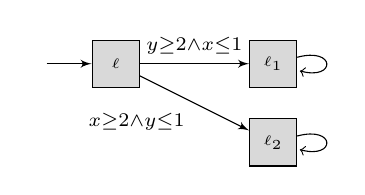
\begin{tikzpicture}[node distance=2cm,auto]
  \tikzstyle{every state}=[rectangle,fill=black!15,minimum size=17pt,inner sep=0pt]
  \everymath{\scriptstyle}
  \node (preA) at (0,0) {};
  \node[state] at (1,0) (A) {\texttt{\scriptsize $\ell$}};
  \node[state,right of=A] (B) {\texttt{\scriptsize $\ell_1$}};
  \node[state,below of=B, node distance=1cm] (C) {\texttt{\scriptsize $\ell_2$}};
  \path[-latex'] 
    (preA) edge (A)
    (A) edge node[above] {$y\geq 2\land x\leq 1$} (B)
    (A) edge node[below left] {$x\geq 2\land y\leq 1$} (C)
    (B) edge[loop right] (B)
    (C) edge[loop right] (C);
\end{tikzpicture}
\qquad
  \tikz{
    \begin{scope}[scale=.4]
      \fill[gray] (0,2) -- (1,2) -- (1,3.2) -- (0,3.2) -- cycle;
      \fill[gray] (0,1) -- (1,2) -- (0,2) -- cycle;
      \fill[gray] (2,0) -- (2,1) -- (3.2,1) -- (3.2,0) -- cycle;
      \fill[gray] (1,0) -- (2,1) -- (2,0) -- cycle;
      \draw[-latex',line width=.6pt] (0,0) -- (3.5,0) node[right] {$x$};
      \draw[-latex',line width=.6pt] (0,0) -- (0,3.5) node[left] {$y$};
      \begin{scope}[line width=0.1pt]
      \draw[-] (1,0) -- (1,3.5);
      \draw[-] (2,0) -- (2,3.5);
      \draw[-] (0,1) -- (3.5,1);
      \draw[-] (0,2) -- (3.5,2);
      \draw[-] (0,0) -- (3.5,3.5);
      \draw[-] (1,0) -- (3.5,2.5);
      \draw[-] (2,0) -- (3.5,1.5);
      \draw[-] (0,1) -- (2.5,3.5);
      \draw[-] (0,2) -- (1.5,3.5);
    \end{scope}
    \end{scope}
    }

Thus, we will represent our states as sets of DBMs given for each location of
the timed game, which will represent the union of convex sets for each location.

All operations that we defined in the previous section can be computed
using unions of DBMs.
\begin{theorem}[\cite{Cassez05}]
  For any DBM~$M$, and edge~$e$, $\post_e([M])$ can be computed as a DBM.
  Furthermore, for any $X\subseteq \calQ$ given as a union of DBMs, 
  $\pi(X)$ can be computed as a union of DBMs.
\end{theorem}

We will not give the details of the successor and predecessor computations using
DBMs, which would allow to prove the theorem above. We refer the interested reader 
to the survey~\cite{bengtsson2004timed} for the details. In the rest of this
paper, we assume blackbox procedures are given for successor and controllable 
predecessor computation. 

\section{Backward Algorithm}
Given a timed game~$\TA$ and safety specification~$B \subseteq \calQ$ given as a
DBM, the \emph{backward synthesis algorithm} simply consists in iteratively
computing the fixpoint of the operator~$\pi$, that is, $\pi^*(\calQ\setminus
B)$.

Moreover, given $W = \pi^*(\calQ\setminus B)$, a winning strategy~$f$ is given
by choosing, for each~$q \in W$, $(d,e) \in \Realnn \times E_c$ which witnesses
that~$q \in \pi(W)$. Such a choice exists since $W = \pi(W)$.
Such a function can be computed by redefining $\predt$ to keep the witness delay
as follows.
\[
  \begin{array}{rl}
    \predt^w(X,Y) = \{&(q,d) \in \calQ \times \Realnn \mid q+d \in X,\\
      & \land \forall d' \in[0,d), q+d' \not \in Y\}.
  \end{array}
\]
Accordingly, we define
\[
  \pi^w(X) = \bigcup_{e \in E_c} \{ (q,d,e) \mid 
      \predt^w(\predc^e(X), \predu(\calQ \setminus X)),
\]
where $\predc^e(X)$ is the predecessors along the edge~$e$ only.
$\pi^w(X)$ is now a set of triples $(q,d,e)$ such that from~$q$,
the controller can delay~$d$ and take transition~$e$ to guarantee ending in~$X$.
It can be shown that the projection of $\pi^w(X)$ into the first component is
exactly~$\pi(X)$ (see \cite{Cassez05}).
Moreover, $\pi^w(X)$ can also be represented by a union of DBMs.

We summarize the computation in the following algorithm. After having computed
the fixpoint, we just check whether the initial state $(\ell_0,\vec{0})$ is
in the fixpoint. If not, then there is no winning control strategy, which means
that the specification is not realizable. Otherwise, we return the winning
strategy.

It is also possible to break the while loop whenever the initial state is
outside~$W$.
\begin{algorithm}
   \small
   Given timed automaton~$\TA$ and set~$B\subseteq \calQ$\;
   $W := \calQ \setminus B$\;
   \While{$W \neq \pi(W)$}{
    $W$ := $\pi(W)$\;
   }
   \eIf{$(\ell_0,\vec{0}) \not \in W$}{
     Return UNREALIZABLE\;
    }{
      Return $\pi^w(X)$\;
    }
   \caption{Backward synthesis algorithm}
\end{algorithm}

\section{Forward Algorithm}
\label{section:forward}
Although the backward algorithm solves the problem of controller synthesis, it
has some disadvantages. 
First of all, it represents the states as
unions of DBMs, and it is difficult to bound the number of DBMs occurring in
each union in practice. Thus, the size of this representation can grow, and
render the synthesis highly inefficient.
Moreover, the backward algorithm requires to compute the \emph{largest}
fixpoint of the operator~$\pi$, even though a much smaller fixpoint might
exist, \textit{i.e.}
a set~$S\subseteq \calQ$, which
contains the initial state ($(\ell_0,\vec{0}) \in S$), and satisfying $S \subseteq
\pi(S)$. In this case, one can derive a controller from~$S$ to avoid~$B$.
It turns out that this does happen in practice; in several situations
there exist simple controllers that are able to control the system in few steps
(thus, they use a small fixpoint~$S$).
Moreover, if we can find such a set~$S$ quickly, then the unions
of DBMs might grow less, and their sizes might stay manageable.

In this section, we present a \emph{forward} algorithm in order to find a
smaller fixpoint to the operator~$\pi$.
The algorithm was presented in~\cite{Cassez05}, and
is an adaptation of~\cite{LiuS98} to timed games.

The basic idea is to start in the initial state, and run a depth-first search 
of the state space using the $\post_e$ operator. Moreover, whenever a state
intersecting~$B$ is encountered, we go back along the search prefix 
to compute those states from which the controller cannot avoid entering~$B$, using the operator~$\pi$. 
If the initial state is in this case, we declare the system uncontrollable.
Otherwise, we continue the exploration. Whenever we reach a fixpoint, this means that
the controller has a winning strategy, which can be extracted from the search
tree.

For the details of the algorithm, we refer to~\cite{Cassez05}.

\section{Software Tools}
Several academic tools have been developed for synthesizing controllers using the timed
automaton formalism.
The first tools were SynthKro and FlySynth developed within the Kronos model
checker framework~\cite{altisen2002tools}. The first one implemented the
backward algorithm using additional tricks to avoid computing the complement of
DBMs; while the latter one implemented a ``semi-on-the-fly'' algorithm based on
two phases. In the first phase, the tool analyzes the timed automaton and
produces a finite automaton that is \emph{time-abstract bisimilar}, that is,
bisimilar with possibly different timing delays. Once this finite game is
produced, then an on-the-fly algorithm is applied to solve it; and any winning
strategy in the finite game is mapped to a winning strategy in the timed game.
The binary executables of SynthKro are still available from
\url{www-verimag.imag.fr/DIST-TOOLS/TEMPO/kronos/} although it has not been
maintained since 2002.

A widely known and maintained tool is UPPAAL-TIGA, which is an extension of the timed automata
model checker UPPAAL to solve timed games. This tool implements the on-the-fly algorithm
we sketched in Section~\cref\{section:forward} from~\cite{Cassez05}. The tool comes with a graphical
user interface which allows one to draw timed automata, compose them in
parallel, and also use bounded integer variables and arrays to construct
systems. A new version of the tool called UPPAAL-STRATEGO was released recently,
which allows one to first synthesize strategies, and then optimize them using
statistical simulation techniques. One can thus obtain strategies both with hard
guarantees (the safety condition will always be satisfied), and soft guarantees
obtained by statistical simulation.
The tools are not open source but freely available for academic purposes. They
can be downloaded, respectively, from
\url{http://people.cs.aau.dk/~adavid/tiga/}
and \url{http://people.cs.aau.dk/~marius/stratego/}.

An open-source tool called Synthia uses similar ideas to solve timed games but applies
an additional abstraction refinement procedure in order to cope with timed
automata that have large discrete parts (that is, when the underlying finite
automaton is already very large). The tool and its sources are available from
\url{https://www.react.uni-saarland.de/tools/synthia/}.

\section{Solution of the Example}
We used the tool UPPAAL-TIGA to compute a controller for the railroad switch
example described in the introduction. The tool outputs a detailed description
of the strategy, prescribing the action to take at each discrete state, and
given clock constraints. The full strategy is given in the appendix. 

We will look at the strategy in some critical states. The strategy contains the
following actions.

{\scriptsize
\begin{verbatim}
State: ( TER.crossing TGV.arrived ) 
When you are in (y<=1), take transition 
          TGV.arrived->TGV.stopping { y <= 1, tau, 1 }
While you are in	(2<=y), wait.
\end{verbatim}
}

Here, if the TER is currently crossing the switch, and if TGV has arrived, then
the strategy stops the TGV, provided that~$y\leq 1$. Note that upon arrival to
the stopping state, the clock~$y$ is reset, so the strategy is always able to
stop the TGV. The second line prescribes to wait if~$y\geq 2$, but this state
will actually not be reached, as the first case is always enabled.\footnote{Note
that the strategy synthesized by UPPAAL prescribes actions from all states,
and not only from those states that are guaranteed to be reached. Note that
we also defined a strategy as a total function from~$\calQ$ to actions.}

What happens if both trains have arrived to the switch? The strategy prescribes
the following actions.

{\scriptsize
\begin{verbatim}
State: ( TER.arrived TGV.arrived ) 
While you are in	(1<x && 2<y) || (1<x && y==2 && x<=2) || 
              (2<=x && 1<y && y<=2 && y<x), wait.
When you are in (1<y && x<=1), take transition 
              TER.arrived->TER.stopping { x <= 1, tau, 1 }
When you are in (y<=1), take transition 
              TGV.arrived->TGV.stopping { y <= 1, tau, 1 }
\end{verbatim}
}

In the first case, we do nothing since it is too late to stop both trains. This
case will never happen if we follow the strategy from the initial state.
In the second case, we stop the TER, since there is still time ($x\leq 1$)
although we cannot stop the TGV ($1<y$). In the third case, we stop the TGV
since $y\leq 1$.

\medskip

Note that the computed strategy actually stops all trains before letting them
go, even though the other train is idle. If we want to avoid stopping the
trains, one can strengthen the objective, and require for instance that both
trains must not be stopping at the same time, and that if one is idle, the other
one should not be stopping etc. Perhaps a more natural way would be to compute
an \emph{optimal} strategy, which minimizes the number of times the stopping
state is visited. Such problems can be modeled by assigning costs to states.
Although the exact decision problem of optimal controller synthesis in timed
games is undecidable~\cite{BBR-formats01}, UPPAAL-STRATEGO could be used to
first compute the set of winning strategies for the safety objective, and then
minimize the cost by statistical simulation. 


\section{Conclusion}
We introduced controller synthesis algorithms for timed automata models, using
the difference-bound matrix representation for the state space.
We first summarized the backward fixpoint computation for solving finite-state
games, and extended it to solve timed games. We also described a forward algorithm
that finds smaller fixpoints and terminates faster in practice. 
Note that both in verification and controller synthesis backward and forward
algorithms are complementary and each can yield a better performance depending
on the model. 

Note that it is also possible to verify or synthesize timed automata using
\emph{discrete-time}, \textit{i.e.} when the allowed timed delays are only
natural numbers. One problem with the discrete time is that one may have to
choose and fix a granularity for the time delays (should the controller observe
the system every second, or every millisecond?). Choosing smaller granularities
can significantly worsen the running time of the algorithms. Moreover, if the
system interacts with a physical environment which has a much more precise
granularity (say, a human user using a system with granularity 1 second) then
the uncontrollable events the environment may send will not be reacted to
immediately. 
Continuous-time semantics (as used in this tutorial) is often a good choice 
since it is a good abstraction for an unknown granularity, and moreover one can
model arbitrarily precise environments.

Nevertheless, there are several situations where discrete time largely suffice for
verification or synthesis purposes. In this case, one can always encode timed
automata seeing the clocks as variables with finite domain, and use well-known
verification techniques, for instance, using binary decision
diagrams (BDD)~\cite{bozga1999efficient,beyer2001efficient}.
A rule of thumb is that such techniques are efficient when the discrete part
(\textit{i.e.} the locations) is already big, and when the timing constraints
are simple and use rather small constants. These techniques are in general
sensitive to big constants used in the guards, and the performance is seriously impaired
when one uses larger constants.

A common feature of both DBM-based algorithms we presented here is that, unlike
BDD-based algorithms, they
explicitly enumerate the discrete part of the model. In other terms, the
locations are visited one by one, while DBMs compactly represent large sets of clock 
valuations which can occur in a given location. In general, techniques based on
DBMs for timed automata are efficient when the number of locations is rather
small, and timing constraints nontrivial. These algorithms are much less
sensitive to the size of the constants; in particular, the exact same
performance is obtained when one multiplies all constants by, say, 1000,
although discrete-time algorithms will most probably fail.

There are several efforts to define efficient data structures to combine both
ideas so that both the discrete parts and the timings constraints can be
represented compactly. \emph{Clock difference
diagrams}~\cite{behrmann1999efficient}, \emph{clock restriction
diagrams}~\cite{wang2002symbolic}, and \emph{constraint matrix
diagrams}~\cite{ehlers2010fully} are some examples of these data structures. A major
challenge in this setting is to find a good compromise between compactness
and computational efficiency.

In conclusion, this tutorial presented one aspect of controller synthesis for
timed systems. We believe a controller synthesis practitioner or enthusiast
should master various formalisms, understand the basics of several
algorithms, and have a feeling of which algorithm could work in which case.

\section*{Acknowledgment}

The author is supported by the ERC starting grant inVEST (FP7-279499).


\bibliographystyle{IEEEtran}
\bibliography{references} 
\appendix
We used UPPAAL-TIGA to synthesize a strategy for the example of
Fig.~\cref\{fig:ter}-\cref\{fig:tgv} for the objective
{\small
\begin{verbatim}
control: A[] not (TER.crossing and TGV.crossing)
\end{verbatim}
}
\noindent which means that both models should never be at the crossing state at the same
time.
The tool answers that there exists a strategy to satisfy this objective, and
outputs the following one.
\scriptsize
\begin{verbatim}
State: ( TER.close TGV.crossing ) 
While you are in	true, wait.

State: ( TER.close TGV.idle ) 
While you are in	true, wait.

State: ( TER.crossing TGV.arrived ) 
When you are in (y<=1), take transition 
          TGV.arrived->TGV.stopping { y <= 1, tau, 1 }
While you are in	(2<=y), wait.

State: ( TER.stopping TGV.arrived ) 
While you are in	(1<y && y<2), wait.
When you are in (y<=1), take transition 
        TGV.arrived->TGV.stopping { y <= 1, tau, 1 }
When you are in (2<=y), take transition 
        TER.stopping->TER.crossing { 1, tau, x := 0 }

State: ( TER.crossing TGV.idle ) 
While you are in	true, wait.

State: ( TER.stopping TGV.stopping ) 
When you are in true, take transition 
        TGV.stopping->TGV.crossing { 1, tau, y := 0 }

State: ( TER.crossing TGV.close ) 
While you are in	true, wait.

State: ( TER.idle TGV.close ) 
While you are in	true, wait.

State: ( TER.arrived TGV.crossing ) 
While you are in	(2<=x), wait.
When you are in (x<=1), take transition 
      TER.arrived->TER.stopping { x <= 1, tau, 1 }

State: ( TER.idle TGV.crossing ) 
While you are in	true, wait.

State: ( TER.close TGV.stopping ) 
When you are in true, take transition 
      TGV.stopping->TGV.crossing { 1, tau, y := 0 }

State: ( TER.arrived TGV.idle ) 
While you are in	(1<x), wait.
When you are in (x<=1), take transition 
      TER.arrived->TER.stopping { x <= 1, tau, 1 }

State: ( TER.close TGV.close ) 
While you are in	true, wait.

State: ( TER.idle TGV.arrived ) 
While you are in	(1<y), wait.
When you are in (y<=1), take transition 
      TGV.arrived->TGV.stopping { y <= 1, tau, 1 }

State: ( TER.arrived TGV.stopping ) 
When you are in (x<=1) || (2<=x), take transition 
        TGV.stopping->TGV.crossing { 1, tau, y := 0 }
While you are in	(1<x && x<2), wait.

State: ( TER.idle TGV.idle ) 
While you are in	true, wait.

State: ( TER.stopping TGV.crossing ) 
While you are in	true, wait.

State: ( TER.stopping TGV.idle ) 
When you are in true, take transition 
        TER.stopping->TER.crossing { 1, tau, x := 0 }

State: ( TER.arrived TGV.arrived ) 
While you are in	(1<x && 2<y) || (1<x && y==2 && x<=2) 
                    || (2<=x && 1<y && y<=2 && y<x), wait.
When you are in (1<y && x<=1), take transition 
              TER.arrived->TER.stopping { x <= 1, tau, 1 }
When you are in (y<=1), take transition 
              TGV.arrived->TGV.stopping { y <= 1, tau, 1 }

State: ( TER.arrived TGV.close ) 
While you are in	(1<x), wait.
When you are in (x<=1 && x<=y) || (x<=1 && y<x), take transition 
              TER.arrived->TER.stopping { x <= 1, tau, 1 }

State: ( TER.stopping TGV.close ) 
When you are in true, take transition 
              TER.stopping->TER.crossing { 1, tau, x := 0 }

State: ( TER.close TGV.arrived ) 
While you are in	(1<y), wait.
When you are in (y<=1), take transition 
              TGV.arrived->TGV.stopping { y <= 1, tau, 1 }

State: ( TER.idle TGV.stopping ) 
When you are in true, take transition 
              TGV.stopping->TGV.crossing { 1, tau, y := 0 }

State: ( TER.crossing TGV.stopping ) 
While you are in	true, wait.

\end{verbatim}
\end{document}


